%%%%%%%%%%%%%%%%%%%%%%%%%%%%%%%%%%%%%%%%%%%%%%%%%%%%%%%%%%%%%%%%%%%%%%%%%%%

\documentclass{standalone}

\usepackage{amsmath}
\usepackage{mathptmx}
\usepackage{pgfplots}
\usetikzlibrary{external}
\tikzexternalize{e-12-balance}
\pgfplotsset{compat=1.16}

%% IEEE uses Times Roman font, so we'll default to Times.
%% These three commands make up the entire times.sty package.
\renewcommand{\rmdefault}{ptm}
\renewcommand{\ttdefault}{pcr}
\normalfont\selectfont

\begin{document}

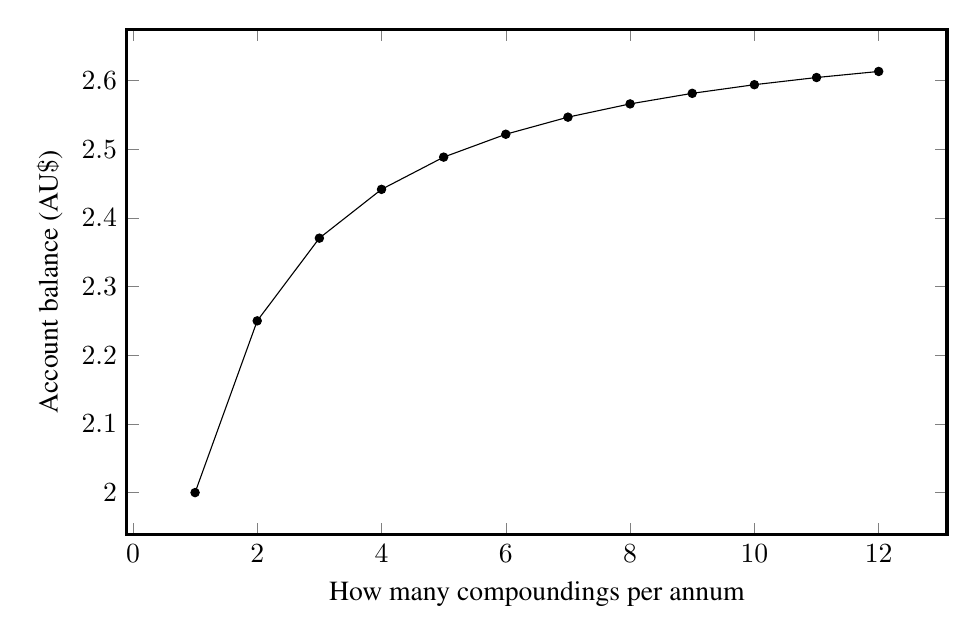
\begin{tikzpicture}
\tikzset{%%
  every mark/.append style={scale=1.0},%%
  scale=1.0%%
}
\pgfplotsset{%%
  every axis/.append style={font=\normalsize}%%
}
%%
\begin{axis}[%%
  axis line style=very thick,%%
  dotStyle/.style={mark size=1.5,black,mark color=black,mark=*},%%
  enlargelimits=true,%%
  height=8cm,%%
  width=12cm,%%
  %% x axis
  xlabel={\normalsize How many compoundings per annum},%%
  %% y axis
  ylabel={\normalsize Account balance~(AU$\$$)}%%
]
%%
%%
\addplot[dotStyle] coordinates {
  (1, 2)
  (2, 2.25)
  (3, 2.37037037037037)
  (4, 2.44140625)
  (5, 2.48832)
  (6, 2.52162637174211)
  (7, 2.54649969704071)
  (8, 2.56578451395035)
  (9, 2.5811747917132)
  (10, 2.5937424601)
  (11, 2.60419901189753)
  (12, 2.61303529022468)
};
\end{axis}
\end{tikzpicture}

\end{document}
